\documentclass[oneside, 11pt]{article}

\usepackage[T1]{fontenc}
\usepackage[utf8]{inputenc}
\usepackage[english]{babel}
\usepackage{enumerate}
\usepackage{isotope}


\usepackage{fouriernc}
\usepackage[detect-all, binary-units, separate-uncertainty=true,
            per-mode=symbol, retain-explicit-plus, retain-unity-mantissa=false]{siunitx}

\usepackage{setspace}
\setstretch{1.2}

\setlength{\parskip}{\smallskipamount}
\setlength{\parindent}{0pt}

\usepackage[headheight=14pt]{geometry}
\geometry{marginparwidth=0.5cm, verbose, a4paper, tmargin=3cm, bmargin=3cm,
          lmargin=2cm, rmargin=2cm}

\usepackage{float}

\usepackage[fleqn]{amsmath}
\numberwithin{equation}{section}
\numberwithin{figure}{section}

\usepackage{graphicx}
\graphicspath{{images/}{../../../images/}}

\usepackage{tikz}
\usetikzlibrary{shapes}
\usetikzlibrary{plotmarks}

\newcounter{Exercise}
\setcounter{Exercise}{1}
\usepackage{xcolor}
\definecolor{shadecolor}{gray}{0.9}
\usepackage{framed}
\usepackage{caption}

\usepackage{url}


\usepackage{fancyhdr}
\pagestyle{fancy}
\fancyhf{}
\rhead{\thepage}
\renewcommand{\footrulewidth}{0pt}
\renewcommand{\headrulewidth}{0pt}

\fancypagestyle{firststyle}
{
    \fancyhf{}
    \rhead{\thepage}
    \cfoot{\includegraphics[height=30pt]{HiSPARClogo}}
    \rfoot{\includegraphics[height=25pt]{CCbysa}}
    \lfoot{
\includegraphics[height=30pt]{NIKHEFlogo}}
    \renewcommand{\footskip}{50pt}
    \renewcommand{\footrulewidth}{0.1pt}
    \renewcommand{\headrulewidth}{0pt}
}

\newcommand{\figref}[1]{Figuur~\ref{#1}}

\newcommand{\hisparc}{\textsmaller{HiSPARC}\xspace}
\newcommand{\kascade}{\textsmaller{KASCADE}\xspace}
\newcommand{\sapphire}{\textsmaller{SAPPHiRE}\xspace}
\newcommand{\jsparc}{\textsmaller{jSparc}\xspace}
\newcommand{\hdf}{\textsmaller{HDF5}\xspace}
\newcommand{\aires}{\textsmaller{AIRES}\xspace}
\newcommand{\csv}{\textsmaller{CSV}\xspace}
\newcommand{\python}{\textsmaller{PYTHON}\xspace}
\newcommand{\corsika}{\textsmaller{CORSIKA}\xspace}
\newcommand{\labview}{\textsmaller{LabVIEW}\xspace}
\newcommand{\daq}{\textsmaller{DAQ}\xspace}
\newcommand{\adc}{\textsmaller{ADC}\xspace}
\newcommand{\hi}{\textsc{h i}\xspace}
\newcommand{\hii}{\textsc{h ii}\xspace}
\newcommand{\mip}{\textsmaller{MIP}\xspace}
\newcommand{\hisparcii}{\textsmaller{HiSPARC II}\xspace}
\newcommand{\hisparciii}{\textsmaller{HiSPARC III}\xspace}

\DeclareSIUnit{\electronvolt}{\ensuremath{\mathrm{e\!\!\:V}}}

\DeclareSIUnit{\unitsigma}{\ensuremath{\sigma}}
\DeclareSIUnit{\mip}{\textsmaller{MIP}}
\DeclareSIUnit{\adc}{\textsmaller{ADC}}

\DeclareSIUnit{\gauss}{G}
\DeclareSIUnit{\parsec}{pc}
\DeclareSIUnit{\year}{yr}



\begin{document}

\title{Radiotelescopen}
\author{N.G. Schultheiss}
\date{}

\maketitle
\thispagestyle{firststyle}

\section{Inleiding}

In de module ``Het uitdijend Heelal'' hebben we gezien dat het heelal
steeds groter wordt. Bijgevolg zijn de lichtstralen van melkwegstelsels
die ver van ons af staan naar het rood verschoven. Extreem verre sterren
hebben een extreme verschuiving. In het microgolf gebied (zeer korte
radiostraling) kunnen we de kosmische achtergrondstraling van de Big
Bang waarnemen. Deze straling is verdeeld als een zwarte straler
\footnote{Wilhelm Carl Werner Otto Fritz Franz Wien (1864-1928)
onderzocht hoe de verdeling van de kleuren van het licht / golflengten
van het licht was bij voorwerpen die warm worden gemaakt. Om de kleur
van het voorwerp niet mee te laten tellen gebruikte hij zwarte
voorwerpen. Als deze gloeiend heet wordt geven ze dus wel licht. Als je
er echter licht licht op laat vallen wordt al het licht geabsorbeerd. In
de praktijk kun je een zwarte straler goed maken door een gaatje in een
blok te boren. Het gat kun je als zwarte straler zien. Al het licht
wordt door het zwarte gat geabsorbeerd. Het is wel handig om de wanden
van het gat zwart te maken met bijvoorbeeld roet van een kaars. Koude
voorwerpen stralen alleen (ver) infrarood licht uit.} met een maximum
bij een golflengte van 6cm.


\section{De opstelling}

\begin{figure}[h]
\noindent \begin{centering}
\includegraphics[width=10cm]{Westerbork_Radio_Telescoop}
\par\end{centering}

\caption{Schotels in Westerbork\cite{westerbork}}
\end{figure}


De eerste opstellingen voor radioastronomie werden na de tweede oorlog
gebouwd in Westerbork uit overtollige radarapparatuur van de tweede
wereldoorlog. Nu is een opstelling eventueel te bouwen met overtollige
satellietontvangers. De radiosignalen voor satellietontvangst ligt
in de orde van 12GHz.


\paragraph*{Opdracht 1:}

\emph{Bereken de golflengte van het satellietsignaal en leg uit of
met satellietschotels aan radioastronomie kan worden gedaan.}

Een nadeel van radioastronomie is dat een radiosignaal een veel grotere
golflengte heeft dan licht. Om een opstelling met een goede resolutie
te bouwen hebben we dus een heel grote paraboolspiegel nodig. In de
module ``Telescopen'' hebben we gezien dat de resolutie te vinden
is door de golflengte van het signaal te delen door de diameter van
de spiegel.

In de radioastronomie zet men meestal een aantal schotels op een lijn.
Samen werken deze schotels als een grote schotel. Met een aantal satellietschotels
is op school ook radioastronomie te bedrijven. Met drie schotels en
ontvangers is al wat te doen. Deze schotels zijn met kabels aan een
meetstation te koppelen. De lengte van de kabel is van belang omdat
gelijktijdige signalen van de schotels ook gelijktijdig in het meetcentrum
moeten komen. Het radiosignaal gaat bij benadering met de lichtsnelheid
door de atmosfeer. Helaas gaat het signaal ongeveer 1,5 maal zo langzaam
door een coaxkabel. De kabels moeten dus precies evenlang zijn voor
iedere schotel. Verder is het noodzakelijk om één soort kabels te
gebruiken. Als we de signaalsterkte van het signaal van de schotels
kunnen meten hebben we al een soort radiotelescoop.


\paragraph*{Opdracht 2:}

\emph{Onderzoek op internet wat er nodig is voor een eenvoudige radiotelescoop
en hoe je deze kunt bouwen.}


\section{De resolutie van een radiotelescoop}

Volgens de module ``Telescopen'' kunnen we de resolutie van één
schotel vinden met:

\begin{equation}
\sin(\alpha)\approx \tan(\alpha)\approx\frac{\lambda}{Diameter}
\end{equation}


Voor een golflengte van 2,5cm en een schoteldiameter van 50cm komen
we op een hoek van:

\begin{equation}
\sin(\alpha)\approx \tan(\alpha)\approx\frac{\mathrm{2,5cm}}{50\mathrm{cm}}=0,050
\end{equation}


De maximale hoek ligt dus in de orde van $2,9^{\mathrm{o}}$ of $0,050$
radialen.


\paragraph*{Opdracht 3:}

\emph{Deze gevoeligheid is ook te bepalen door de schotel op een satelliet
te richten. Daarna is te kijken wanneer het satellietsignaal wegvalt
als de schotel wordt verdraaid.}

De resolutie van een radiotelescoop kan worden verhoogd door een aantal
detectoren tegelijk te gebruiken. Dit kan door de detectoren in een
lijn op te stellen.

\begin{figure}[H]
\noindent \begin{centering}
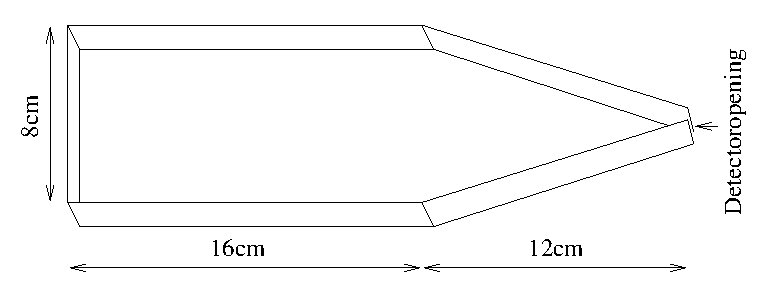
\includegraphics{opstelling}
\par\end{centering}

\caption{Een opstelling met twee detectoren}
\end{figure}


In figuur 3.1 zien we een radiosignaal loodrecht op de opstelling
af komen. De detectoren meten een synchroon signaal, dat wil zeggen
dat de spanning van de detectoren tegelijk op en neer gaat. Om een
zo klein mogelijk deel van de hemel te meten, willen we de schotels
daarom zo ver mogelijk uit elkaar zetten. Er zijn echter meerdere
manieren om synchrone signalen te detecteren.

\begin{figure}[H]
\noindent \begin{centering}
\includegraphics{opstelling1}
\par\end{centering}

\caption{Een schuin invallende radiogolf}
\end{figure}


In figuur 3.2 is te zien hoe een radiogolf schuin op de opstelling
invalt. Het radiosignaal legt voor de linkerdetector precies een golflengte
meer af dan voor de rechterdetector. Beide gemeten signalen zijn weer
synchroon. De opstelling is dus ook voor deze hoek extra gevoelig. 


\paragraph*{Opdracht 4:}

\emph{Leg uit of je voor een opstelling die voor kleine hoeken gevoelig
is, de schotels ver uit elkaar of dicht bij elkaar moet zetten.}


\paragraph*{Opdracht 5:}

\emph{Leg uit of het zinvol is om de schotels heel ver uit elkaar
te zetten. Denk aan het weglengteverschil tussen twee schotels!}


\paragraph*{Opdracht 6:}

\emph{Leg uit waarom we drie schotels het beste in de hoekpunten van
een gelijkzijdige driehoek kunnen zetten om de radiosignalen uit een
zo klein mogelijk deel van de hemel te meten.}


\section{Pulsars}

Dame Susan Jocelyn Bell Burnell (1943-) werkte bij professor Hewish
in Cambridge mee aan de constructie van een radiotelescoop. De sterkte
van radiosignaal werd op stroken papier geschreven met een (x,t)-schrijver.
Het was de bedoeling om te ontdekken of er buitenaards leven was (Little
Green Men of LGM). Helaas schreef de recorder veel sneller grafieken,
dan dat Jocelyn Bell de grafieken kon bekijken. Op een gegeven moment
ontdekte ze echter een periodiek signaal. Ergens in het heelal was
iets dat een serie korte radiopulsen uitzond. Zouden dit little green
men zijn?

\begin{figure}[H]
\noindent \begin{centering}
\includegraphics[width=10cm]{plotter}
\par\end{centering}

\caption{Een tweekanaals (x,t)-schrijver}
\end{figure}


De kans dat er op meedere plaatsen in het heelal LGM zouden zijn,
vond ze erg klein. Ze ging daarom op zoek naar andere regelmatige
signalen. Als deze er waren, was er iets anders aan de hand. Na de
berg papier nog eens grondig te hebben bestudeerd, vond ze meerdere
signalen. Het waren dus geen LGM. Er moest iets anders aan de hand
zijn. Een beter idee was dat het een snel rondtollende ster was. Deze
nieuwe ontdekking werd een pulsar genoemd. Een pulsar stuurt als een
soort vuurtoren bundels radiostralen door het heelal. Deze meten we
als een periodiek signaal met een radiotelescoop. Waarschijnlijk zijn
deze pulsars ook een bron voor hoogenergetische kosmische straling. 


\section{Benodigdheden}

Om een interferentie radiotelescoop te bouwen, hebben we de volgende
onderdelen nodig:
\begin{itemize}
\item Een of meerdere schotels.
\item Evenveel LNB \footnote{Een LNB werkt als heterodyne ontvanger voor
satellietsignalen. In een heterodyne ontvanger wordt het antennesignaal
vermenigvuldigd met een middenfrequent signaal. De frequentie van dit
signaal ligt iets boven de helft van de frequentie van het
antennesignaal. Door deze vermenigvuldiging onstaat er een verzameling
van signalen met verschillende frequenties. Met een filter kunnen we de
frequenties voor de UHF (ultra high frequency) en VHF (very high
frequency) band uit deze verzameling halen. Als dit signaal op een TV
wordt aangesloten kunnen we TV-kijken. Omdat de fase van het
antennesignaal en de fase van het middenfrequentsignaal beide belangrijk
zijn voor de fase van het uitgaand signaal, moeten verschillende
schotels in een array eenzelfde middensignaal krijgen. In het ideale
geval is er één middenfrequente bron voor alle schotels van de
opstelling.}'s of Low noise block converters. Deze werken als antenne en
zetten het 12GHz signaal om in een laagfrequenter signaal.
\item Een satellietzoeker, hiermee is de sterkte van het signaal te meten.
\item Coaxkabel en kabelsplitters.
\end{itemize}
Monteer de LNB op de schotel. Via een coaxkabel is de satellietzoeker
aan te sluiten. Let op dat je de satellietzoeker met een impedantie
van $75\Omega$ afsluit. Zonder afsluiting kun je reflecties in je
opstelling krijgen. Met de schotel is nu al te kijken of je een radiobron
kunt waarnemen. Als de schotel iets waarneemt slaat de satellietzoeker
uit. Met een enkele schotel is de Zon goed te zien. Het is al ingewikkelder
om de Maan waar te nemen.

Als volgende stap kan een tweede schotel worden opgesteld. Met een
kabelsplitter kunnen beide schotels waar\-schijn\-lijk op de satellietzoeker
worden aangesloten, dit hangt mede af van het soort LNB's. Met de
satellietzoeker meten we nu de som van de twee signalen. De resolutie
van de opstelling moet hierdoor aanzienlijk toenemen. Let op dat de
kabels van de schotels naar de kabelspitter even lang zijn. Omdat
de golflengte in de orde van 2,5cm is, moet de lengte op de millimeter
kloppen. Een looptijdverschil geeft een fase verschil in de detector
en daarmee een schuine meting.

Tot slot kunnen we via een kabelsplitter een derde schotel toevoegen.
De totale kabellengte, inclusief de lengte van eventuele kabelsplitters
in de kabel, van iedere schotel tot de satellietzoeker moet even groot
zijn. 

\begin{thebibliography}{9}
    \bibitem{westerbork}
        Door Onderwijsgek, \emph{De Westerbork Synthese Radio Telescoop}, CC-BY-SA-2.5-nl, via Wikimedia Commons
\end{thebibliography}

\end{document}
